% =====================================================================
% RESULTS  (borrador generado a partir de results/*.jsonl; revisar antes de pegar)
% Requiere: \usepackage{graphicx}; subir la carpeta figures/ a Overleaf.
% =====================================================================
\section{Results}
\label{sec:results}

All configurations were run once per problem. The prompts and the retrieval query were fixed on the development set, and the
test set was evaluated a single time after the code was frozen. We report pass@1, the fraction of problems whose final
delivered proof is accepted by the Lean verifier.

\subsection{Overall performance}
Table~\ref{tab:main} and Fig.~\ref{fig:pass} summarize pass@1. On the 20 test problems every configuration solves few
problems: pass@1 ranges from 0.05 (Baseline A, 1/20) to 0.15 (w/o RAG,
3/20), and the 95\% Wilson intervals overlap almost completely. None of the paired comparisons in
Table~\ref{tab:pairs} is significant after Bonferroni correction (all $p_{\mathrm{adj}} = 1.000$); the largest paired
difference is 1 problem. Pass@1 on the development set was higher (up to 0.60 for the
full system), a gap we analyze in the Discussion.

\begin{table}[t]
\centering
\caption{pass@1 on the development (10) and test (20) problems. The 95\% Wilson interval refers to test. ``Delivered'' is the number of proofs the system presents as correct; false positives (FP) are delivered proofs that Lean rejects. Calls = mean LLM calls per test problem.}
\label{tab:main}
\footnotesize
\setlength{\tabcolsep}{3pt}
\begin{tabular}{lccccrr}
\hline
Config. & Dev & Test & 95\% CI & Deliv. & FP & Calls \\
\hline
Baseline A & 4/10 & 1/20 & [0.01, 0.24] & 1 & 0 & 1.0 \\
Baseline B & 4/10 & 2/20 & [0.03, 0.30] & 20 & 18 & 2.0 \\
w/o RAG & 5/10 & 3/20 & [0.05, 0.36] & 3 & 0 & 9.6 \\
w/o Critic & 4/10 & 2/20 & [0.03, 0.30] & 2 & 0 & 3.0 \\
Full & 6/10 & 2/20 & [0.03, 0.30] & 2 & 0 & 10.2 \\
\hline
\end{tabular}
\end{table}

\begin{table*}[t]
\centering
\caption{Paired comparisons on the test set. ``Only 1st / 2nd'' counts problems solved by only one configuration; $\Delta$ is the difference in pass@1 with a 95\% bootstrap interval; $p$ is the exact McNemar test with Bonferroni correction ($\times$5).}
\label{tab:pairs}
\footnotesize
\setlength{\tabcolsep}{3pt}
\begin{tabular}{lcccc}
\hline
Comparison & Only 1st & Only 2nd & $\Delta$ pass@1 [95\% CI] & $p_{\mathrm{adj}}$ \\
\hline
Full vs.\ w/o RAG & 0 & 1 & -0.05 [-0.15, +0.00] & 1.000 \\
Full vs.\ w/o Critic & 0 & 0 & +0.00 [+0.00, +0.00] & 1.000 \\
Full vs.\ Baseline A & 1 & 0 & +0.05 [+0.00, +0.15] & 1.000 \\
Full vs.\ Baseline B & 0 & 0 & +0.00 [+0.00, +0.00] & 1.000 \\
w/o Critic vs.\ Baseline A & 1 & 0 & +0.05 [+0.00, +0.15] & 1.000 \\
\hline
\end{tabular}
\end{table*}

\begin{figure*}[t]
\centering
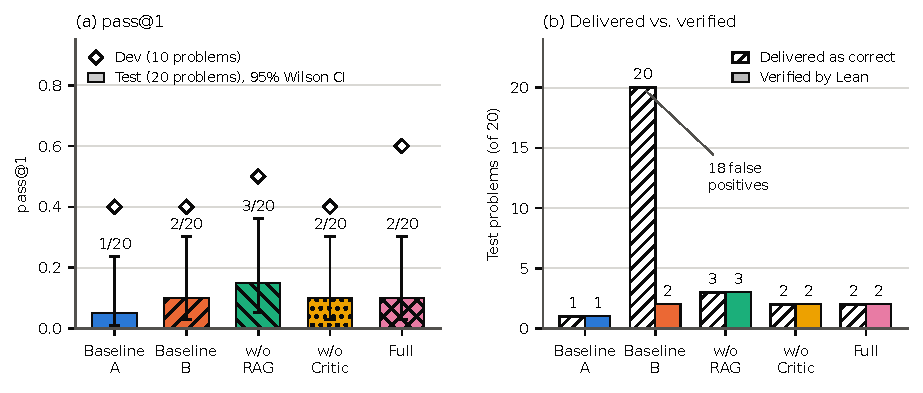
\includegraphics[width=\textwidth]{figures/fig_pass_at_1.pdf}
\caption{(a) pass@1 of the five configurations on the test set with 95\% Wilson intervals; diamonds show pass@1 on the development set. (b) Proofs delivered as correct versus proofs verified by Lean on the test set.}
\label{fig:pass}
\end{figure*}

\subsection{Verification and false positives}
Baseline B generates a natural-language proof, translates it to Lean and delivers it without checking it inside the system.
It therefore delivers all 20 test proofs as correct, but Lean rejects 18 of them (90\%). The
other four configurations use the verifier as the acceptance criterion and delivered no incorrect proof
(Fig.~\ref{fig:pass}b). The same pattern appears on the development set, where Baseline B delivers 10 proofs and
6 are rejected.

\subsection{Per-problem results}
Only 3 distinct test problems were solved by any configuration (Fig.~\ref{fig:problems}):
\texttt{aime\_1989\_p8} by all five configurations, \texttt{mathd\_algebra\_441} by every configuration except Baseline A,
and \texttt{mathd\_numbertheory\_430} only by w/o RAG. No configuration solved any of the 9 intermediate problems
or any of the 7 counting problems (Table~\ref{tab:strata}). On the development set, 6 of the 10 problems were
solved by at least one configuration, all of them basic (\texttt{mathd\_algebra\_141}, \texttt{mathd\_algebra\_33},
\texttt{mathd\_algebra\_398}, \texttt{mathd\_numbertheory\_12}, \texttt{mathd\_numbertheory\_99} and
\texttt{mathd\_numbertheory\_521}); none of the four intermediate or advanced development problems was solved.

\begin{figure*}[t]
\centering
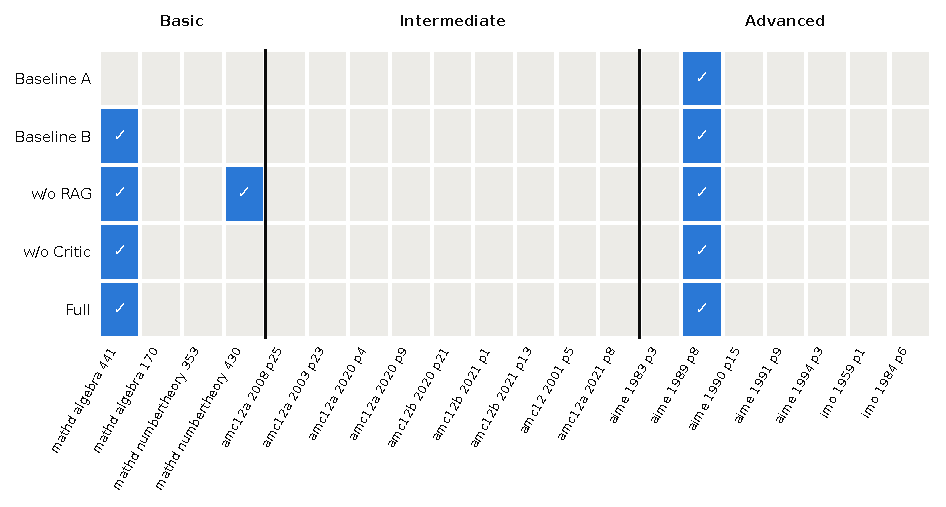
\includegraphics[width=\textwidth]{figures/fig_per_problem.pdf}
\caption{Test problems solved (check mark) by each configuration, grouped by difficulty. Each mark is one problem solved by one configuration, so a problem solved by several configurations is marked in several rows.}
\label{fig:problems}
\end{figure*}

\begin{table}[t]
\centering
\caption{Problems solved by difficulty and by area, on the development and test sets ($n$ = problems in each stratum). The difficulty rows and the area rows count the same problems from two angles, so they are not added together.}
\label{tab:strata}
\footnotesize
\setlength{\tabcolsep}{3pt}
\begin{tabular}{lcccccc}
\hline
Stratum & $n$ & Base A & Base B & w/o RAG & w/o Crit. & Full \\
\hline
\multicolumn{7}{l}{\textit{Development}} \\
Basic & 6 & 4 & 4 & 5 & 4 & 6 \\
Intermediate & 2 & 0 & 0 & 0 & 0 & 0 \\
Advanced & 2 & 0 & 0 & 0 & 0 & 0 \\
Algebra & 5 & 2 & 3 & 3 & 3 & 3 \\
Counting & 2 & 1 & 1 & 1 & 1 & 1 \\
Number theory & 3 & 1 & 0 & 1 & 0 & 2 \\
\hline
\multicolumn{7}{l}{\textit{Test}} \\
Basic & 4 & 0 & 1 & 2 & 1 & 1 \\
Intermediate & 9 & 0 & 0 & 0 & 0 & 0 \\
Advanced & 7 & 1 & 1 & 1 & 1 & 1 \\
Algebra & 6 & 1 & 2 & 2 & 2 & 2 \\
Counting & 7 & 0 & 0 & 0 & 0 & 0 \\
Number theory & 7 & 0 & 0 & 1 & 0 & 0 \\
\hline
\end{tabular}
\end{table}

\subsection{Contribution of the Critic and of retrieval}
Table~\ref{tab:critic} separates problems solved at the first attempt from those solved after retries or replanning. On the
test set, w/o RAG solved 2 problems at the first attempt and 1 after a retry
(\texttt{mathd\_numbertheory\_430}), while the full system solved both of its problems at the first attempt even though it
replanned in 8 of 20 problems (w/o RAG: 6). On the development set, retries rescued
1 problem in w/o RAG and 2 in the full system
(\texttt{mathd\_numbertheory\_99} and \texttt{mathd\_numbertheory\_521}). None of the 4 correct proofs
produced by the configurations with retrieval contains a retrieved lemma.

\begin{table}[t]
\centering
\caption{Contribution of the Critic and of RAG on the test set. A problem is solved at the first attempt if it needed the minimum of three LLM calls (Planner, Generator, AutoFormalizer); more calls imply retries or replanning. The last column counts correct proofs that contain a retrieved lemma.}
\label{tab:critic}
\footnotesize
\setlength{\tabcolsep}{3pt}
\begin{tabular}{lcccc}
\hline
Config. & 1st att. & Retry & Replan & Lemma used \\
\hline
w/o RAG & 2 & 1 & 6 & -- \\
w/o Critic & 2 & 0 & 0 & 0/2 \\
Full & 2 & 0 & 8 & 0/2 \\
\hline
\end{tabular}
\end{table}

\subsection{Cost}
Fig.~\ref{fig:cost} relates pass@1 to cost. The configurations with the Critic need 9.6--10.2 LLM
calls per problem, against 3.0 without the Critic and 1.0--2.0 for the baselines, and
roughly 9.8k--11.7k input tokens per problem, against 2.8k for w/o Critic and
0.3k--1.1k for the baselines. The additional cost is not accompanied by a pass@1 that is
distinguishable from that of the cheaper configurations.

\begin{figure}[t]
\centering
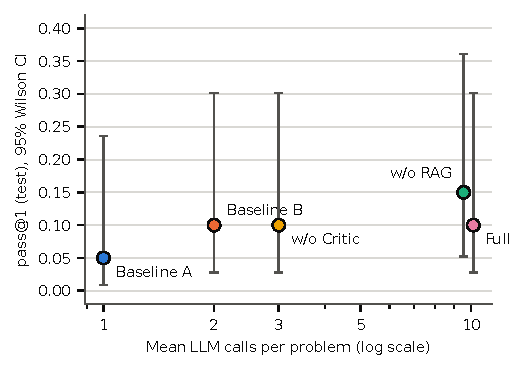
\includegraphics[width=\columnwidth]{figures/fig_cost.pdf}
\caption{pass@1 on the test set versus mean LLM calls per problem (log scale). Bars are 95\% Wilson intervals.}
\label{fig:cost}
\end{figure}

\subsection{Failure analysis}
Table~\ref{tab:errors} and Fig.~\ref{fig:errors} classify the last Lean error of each failed test problem. Failures are
spread over several categories and none disappears when components are added: tactics that do not close the goal
(20 cases across configurations), use of \texttt{sorry} or \texttt{admit} (17;
2--5 per configuration), unknown identifiers (16;
2--4 per configuration) and syntax or formalization errors
(16). The classification is heuristic, based on the last Lean message, so the counts are approximate.

\begin{table}[t]
\centering
\caption{Failure taxonomy on the test set (heuristic classification of the last Lean message of each failed problem).}
\label{tab:errors}
\footnotesize
\setlength{\tabcolsep}{3pt}
\begin{tabular}{lccccc}
\hline
Category & Base A & Base B & w/o RAG & w/o Crit. & Full \\
\hline
Tactic fails & 5 & 3 & 6 & 3 & 3 \\
sorry/admit & 3 & 4 & 2 & 5 & 3 \\
Unknown ident. & 3 & 4 & 4 & 2 & 3 \\
Syntax/formal. & 4 & 2 & 3 & 5 & 2 \\
Timeout/recursion & 2 & 2 & 2 & 1 & 3 \\
Type/instance & 2 & 2 & 0 & 2 & 4 \\
Other & 0 & 1 & 0 & 0 & 0 \\
\textbf{Failed problems} & 19 & 18 & 17 & 18 & 18 \\
\hline
\end{tabular}
\end{table}

\begin{figure}[t]
\centering
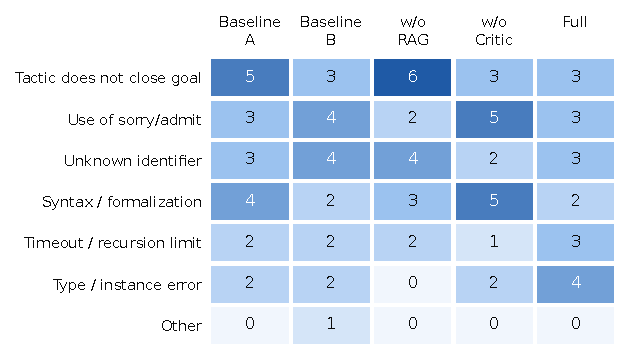
\includegraphics[width=\columnwidth]{figures/fig_errors.pdf}
\caption{Failure taxonomy on the test set (number of failed problems per category and configuration).}
\label{fig:errors}
\end{figure}
